\section*{Consulta 3: Atletas que ganaron más medallas por disciplina y tipo de medalla}

\subsection*{Descripción}
Esta consulta identifica a los atletas que han ganado la mayor cantidad de medallas, clasificadas por disciplina y tipo de medalla. Es útil para evaluar el rendimiento de los atletas en diferentes disciplinas y tipos de medallas.

\textbf{SQL}

\begin{verbatim}
SELECT 
    a.IDAtleta,
    a.Nombre,
    a.PrimerApellido,
    a.SegundoApellido,
    d.NombreDisciplina,
    m.TipoMedalla,
    COUNT(m.TipoMedalla) AS CantidadMedallas
FROM 
    Medalla m
JOIN 
    Atleta a ON m.IDAtleta = a.IDAtleta
JOIN 
    Disciplina d ON m.IDDisciplina = d.IDDisciplina
GROUP BY 
    a.IDAtleta, a.Nombre, a.PrimerApellido, a.SegundoApellido, d.NombreDisciplina, m.TipoMedalla
ORDER BY 
    CASE 
        WHEN m.TipoMedalla = 'Oro' THEN 1
        WHEN m.TipoMedalla = 'Plata' THEN 2
        WHEN m.TipoMedalla = 'Bronce' THEN 3
    END,
    CantidadMedallas DESC;
\end{verbatim}

\begin{center}
    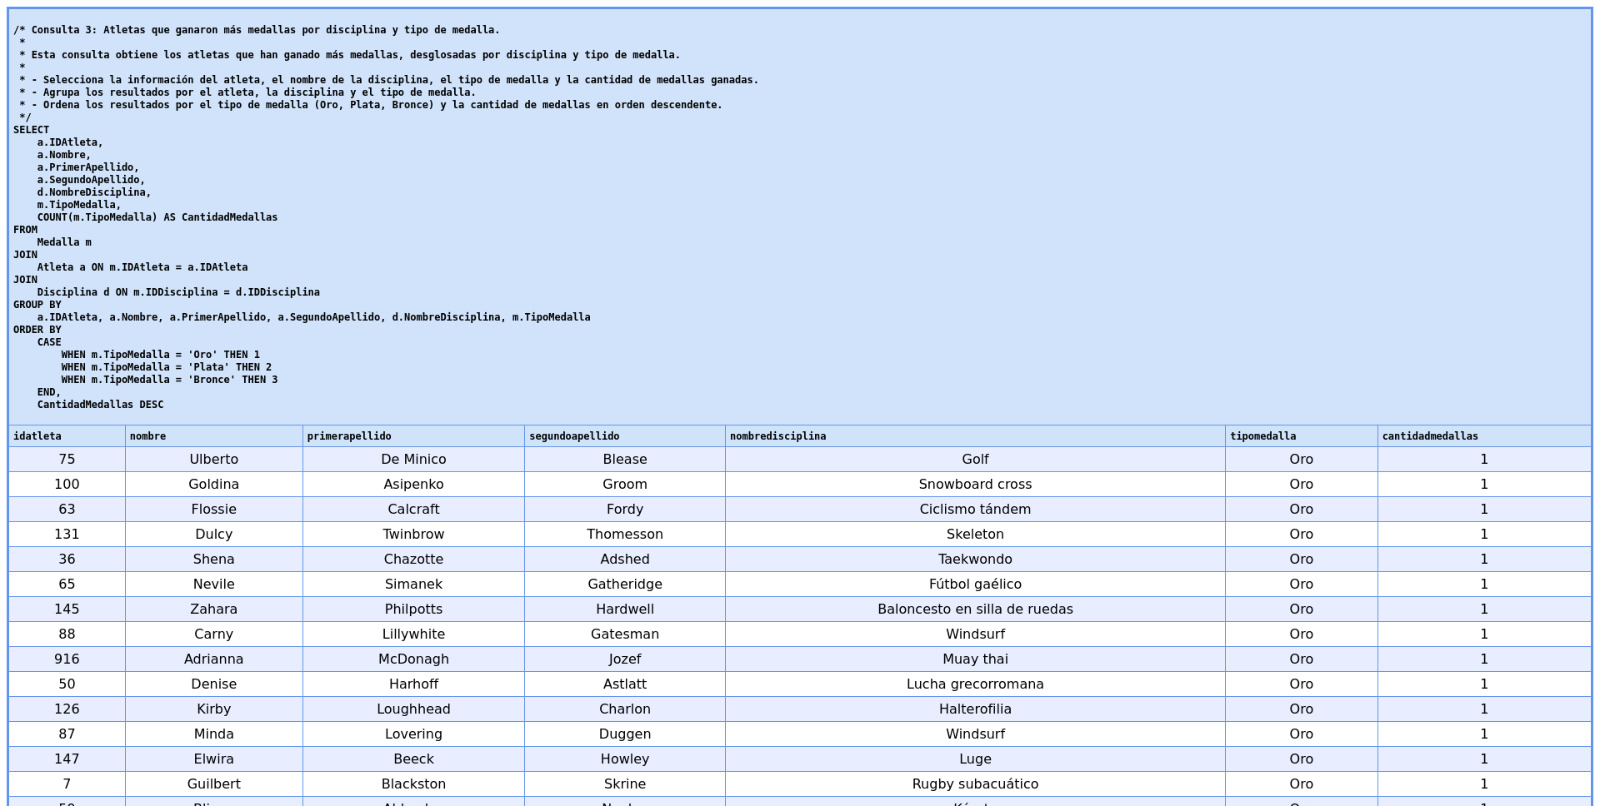
\includegraphics[width=16.5cm]{../resources/Chapters/Consultas/Imagenes/Consulta3.jpeg} 
    
   Consulta 3. Atletas que ganaron más medallas por disciplina y tipo de medalla.
\end{center}

\textbf{Desglose de la consulta}

\begin{itemize}
   \item \textbf{Selección de columnas (\texttt{SELECT})}:
   \begin{itemize}
       \item Se seleccionan las siguientes columnas:
       \begin{itemize}
           \item \texttt{a.IDAtleta}: Identificador único del atleta.
           \item \texttt{a.Nombre}: Nombre del atleta.
           \item \texttt{a.PrimerApellido}: Primer apellido del atleta.
           \item \texttt{a.SegundoApellido}: Segundo apellido del atleta.
           \item \texttt{d.NombreDisciplina}: Nombre de la disciplina.
           \item \texttt{m.TipoMedalla}: Tipo de medalla (Oro, Plata, Bronce).
           \item \texttt{COUNT(m.TipoMedalla)}: Cuenta la cantidad de medallas ganadas, denominada \texttt{CantidadMedallas}.
       \end{itemize}
   \end{itemize}
   
   \item \textbf{Tablas involucradas (\texttt{FROM} y \texttt{JOIN})}:
   \begin{itemize}
       \item La consulta utiliza tres tablas:
       \begin{itemize}
           \item \texttt{Medalla (m)}: Contiene la información de las medallas ganadas.
           \item \texttt{Atleta (a)}: Contiene la información de los atletas.
           \item \texttt{Disciplina (d)}: Contiene la información de las disciplinas.
       \end{itemize}
       \item Se realizan \texttt{JOINs} entre las tablas para relacionar las medallas con los atletas y las disciplinas.
   \end{itemize}
   
   \item \textbf{Agrupación de resultados (\texttt{GROUP BY})}:
   \begin{itemize}
       \item Para calcular la cantidad de medallas ganadas por atleta, disciplina y tipo de medalla, se agrupan los datos según las columnas:
       \begin{itemize}
           \item \texttt{a.IDAtleta}, \texttt{a.Nombre}, \texttt{a.PrimerApellido}, \texttt{a.SegundoApellido}, \texttt{d.NombreDisciplina}, \texttt{m.TipoMedalla}.
       \end{itemize}
       \item Esto garantiza que se genere un registro único por cada combinación de atleta, disciplina y tipo de medalla.
   \end{itemize}
   
   \item \textbf{Ordenamiento de resultados (\texttt{ORDER BY})}:
   \begin{itemize}
       \item Los resultados se ordenan por el tipo de medalla (\texttt{Oro}, \texttt{Plata}, \texttt{Bronce}) y la cantidad de medallas en orden descendente (\texttt{DESC}), de modo que los atletas con más medallas de oro aparezcan primero.
   \end{itemize}
\end{itemize}

\textbf{Análisis detallado}

\begin{enumerate}
   \item \textbf{Relación entre tablas:}
   \begin{itemize}
       \item La consulta asume que existe una relación directa entre las tablas \texttt{Medalla}, \texttt{Atleta} y \texttt{Disciplina} a través de las claves foráneas.
       \item Esto implica que:
       \begin{itemize}
           \item Cada medalla está asociada con un atleta y una disciplina.
           \item Cada atleta puede haber ganado una o más medallas en diferentes disciplinas.
       \end{itemize}
   \end{itemize}
   
   \item \textbf{Uso de la función agregada \texttt{COUNT}:}
   \begin{itemize}
       \item La función \texttt{COUNT(m.TipoMedalla)} cuenta el número de medallas ganadas por cada atleta en cada disciplina y tipo de medalla.
       \item Si un atleta no ha ganado medallas en una disciplina específica, no aparecerá en los resultados porque el \texttt{JOIN} elimina las filas sin coincidencias.
   \end{itemize}
   
   \item \textbf{Agrupación por atleta, disciplina y tipo de medalla:}
   \begin{itemize}
       \item El uso de \texttt{GROUP BY} permite agrupar los registros por atleta, disciplina y tipo de medalla, asegurando que la cantidad de medallas se calcule correctamente para cada combinación.
   \end{itemize}
   
   \item \textbf{Ordenamiento:}
   \begin{itemize}
       \item El orden por tipo de medalla (\texttt{Oro}, \texttt{Plata}, \texttt{Bronce}) y descendente por \texttt{CantidadMedallas} facilita la identificación de los atletas con mayor número de medallas de oro, seguidos por los de plata y bronce.
   \end{itemize}
\end{enumerate}

\textbf{Consideraciones}

\begin{itemize}
   \item \textbf{Empates en la cantidad de medallas:}
   \begin{itemize}
       \item Si varios atletas tienen la misma cantidad de medallas de un tipo específico, el orden relativo entre ellos no está definido. Para resolver esto, se podría agregar un criterio adicional en el \texttt{ORDER BY}, como el nombre del atleta.
   \end{itemize}
\end{itemize}
